
\documentclass[11pt,titlepage,a4paper]{report}

%INCLUSIONE PACCHETTI
%---------------------------------------------
\usepackage[italian]{babel}
\usepackage{fancyhdr}
\usepackage{graphicx}
\graphicspath{{./pics/}}    % cartella di salvataggio immagini

% STILE DI PAGINA
%---------------------------------------------
\pagestyle{fancy}
\renewcommand{\sectionmark}[1]{\markright{\thesection.\ #1}}
\lhead{\nouppercase{\rightmark}}
\rhead{\nouppercase{\leftmark}}
\renewcommand{\chaptermark}[1]{%
\markboth{\thechapter.\ #1}{}}

%Ridefinisco lo stile plain della pagina
\fancypagestyle{plain}{%
	\lhead{
\includegraphics[height=50pt]{logo.eps}}
	\chead{}
	\rhead{HappyCode inc \\ happycodeinc@gmail.com}
	\lfoot{BR-jsys}
	\rfoot{\dt - \lv}
	\cfoot{\thepage}
	\renewcommand{\headrulewidth}{5pt}
	\renewcommand{\footrulewidth}{0.4pt}
}


\begin{document}


%definizione variabili 
\newcommand{\lv}{ 0.5 } % latest version
\newcommand{\dt}{ Specifica Tecnica }% Document title
\newcommand{\Glossario}{ Glossario.1.4.pdf }
\newcommand{\br}{ business rule }
\newcommand{\brs}{ business rules }
\newcommand{\bo}{ business object }
\newcommand{\bos}{ business objects }
\newcommand{\re}{ repository }
\newcommand{\brp}{ BusinessRuleParser }
\newcommand{\brl}{ BusinessRuleLexer }
\newcommand{\BR}{ BusinessRule }
%fine definizione variabili


\hyphenation{glos-sa-rio es-pli-ci-to ve-ri-fi-ca-re re-po-si-to-ry se-gna-la-ta coe-ren-za}
\begin{titlepage}\begin{center}
\vspace*{0.5in}

\includegraphics{logo.eps}
\vspace*{0.2in} \\
{\Large \textbf{BR-jsys}}
{\Large \emph{business rules} per sistemi gestionali in architettura J2EE } 
\vspace{2in} \\
\Huge \textsc{ \dt }
\par\rule{10cm}{0.4pt} \par {\large Versione \lv - \today} \\
\end{center}\end{titlepage}
\vspace*{0.5in}


\begin{center}
\thispagestyle{plain}
\begin{table}[htbp]
\large{
\begin{tabular}{l}
\Large{\textbf{\textsf{Capitolato: ''BR-jsys``}}} \\
\begin{tabular}{||p{6cm}||p{6cm}||} \hline
\textbf{Data creazione:} & 18/11/2007 \\ \hline
\textbf{Versione:} & \lv \\ \hline
\textbf{Stato del documento:} & formale, esterno \\ \hline
% ----------------------------------------------------------------------------autori
\textbf{Redazione:} & Alessia Trivellato ­18/11/2007 \\ \hline
\textbf{Revisione:} &    \\ \hline
\textbf{Approvazione:}  & \\ \hline
\end{tabular} \\
\end{tabular}
}
\end{table}
\begin{table}[hbtp]
\large{
\begin{tabular}{l}
\Large{\textbf{\textsf{Lista di distribuzione}}} \\
\begin{tabular}{||p{6cm}||p{6cm}||} \hline
%  -------------------------------------------------------------lista di distribuzione
{HappyCode inc}& Gruppo di lavoro\\ \hline
{Tullio Vardanega, Renato Conte}& Rappresentanti del committente \\ \hline 
{Zucchetti S.r.l}& Azienda committente\\ \hline
\end{tabular} \\
\end{tabular}
}
\end{table}

\begin{table}[hbtp]
\large{
\begin{tabular}{l}
\Large{\textbf{\textsf{Diario delle modifiche}}} \\
\begin{tabular}{||p{2cm}||p{3.5cm}||p{6cm}||} \hline
%-------------------------------------------------------------------------------diario modifiche
\textbf{Versione} & \textbf{Data rilascio} & \textbf{Descrizione} \\ \hline
0.5 & 05/02/2008 & Aggiunta del nome del file nel modello di documento.\\ \hline
0.4 & 22/01/2008 & Modifica al layout dei documenti.\\ \hline
0.3 & 22/12/2007 & Aggiornamento requisiti. \\ \hline \hline
0.2 & 21/12/2007 & Documento sottoposto a revisionamento automatico.\\ \hline
0.1 & 18/12/2007 & Stesura preliminare del documento. \\ \hline

\end{tabular} \\
\end{tabular}

}
\end{table}
\end{center}
\newpage
\tableofcontents
\chapter{Introduzione}
\section{Scopo del documento}
Il presente documento si ripropone di descrivere il sistema software ``BR-jsys'', sulla base del documento di Analisi dei Requisiti, dal punto di vista architetturale. Lo strumento da noi adottato sar\`a il linguaggio UML, sottoforma di diagrammi delle classi. L'approccio adottato nell'illustrare il sistema sar\`a di tipo ``Bottom-up'' Fornir\`a inoltre una visione pi\`u dettagliata delle componenti da realizzare.
Verr\`a definito il contesto d'uso del sistema e fornita la decomposizione di questo in componenti principali.
\section{Scopo del prodotto}
Per lo scopo del prodotto si faccia riferimento al documento di Analisi dei Requisiti.
\section{Glossario}
Viene fornito come documento esterno chiamato \Glossario .
\section{Riferimenti}
\subsection{Riferimenti normativi}
\begin{itemize}
\item Capitolato d'appalto BR-jsys
\item AnalisiDeiRequisiti
\item NormeDiProgetto
\item PianoDiProgetto
\item PianoDiQualifica
\item ``Ingegneria del software'' 8a edizione - Ian Sommerville 
\item ``The Definitive ANTLR Reference''
\end{itemize}
%Ho tolto i riferimenti informativi

\chapter{Definizione del prodotto}
\subsection{Metodo e formalismo di specifica}
%Copiato di sana pianta dalla Nonsolocodice
Abbiamo attuato la progettazione del prodotto con l'uso di diagrammi UML 2.1 in quanto linguaggio internazionalmente riconosciuto e standardizzato.
Il software di cui l’azienda ha fatto uso per la creazione dei diagrammi e' ArgoUML 0.24. L'utilizzo di tale software deriva dalla completezza
di strumenti di cui e' fornito, i quali soddisfano in pieno le nostre necessita'.

\subsection{Presentazione dell'architettura generale del sistema e identificazione dei componenti architetturali di alto livello}
Lo schema generale del prodotto è specificato nell'immagine sottostante.
%Immagine simile a quella che abbiamo mandato a tullio
Abbiamo deciso di suddividere il prodotto in quattro macrocomponenti:
\begin{enumerate}
 \item \textbf{GUI}:Fornisce all'utente un interfaccia grafica minimale consentendogli di effettuare le operazioni di cancellazione e interrogazione del repository in maniera user-friendly.
\item \textbf{Business Rule}: Componente che rappresenta la \br che l'utente dichiara e che deve essere passata al validatore per compilarla.
\item \textbf{Validatore}: Componente in grado di accettare in input una \br, di validarla, e di inserirla, se scritta correttamente, nel \re.
\item \textbf{Comunicatore}: Componente in grado di connettersi al DBMS esterno e di comunicare con esso tramite i formalismi del linguaggio XQuery.
Sar\`a appunto tramite Query che il DBMS effettuer\`a operazioni di insermento, cancellazione o di ricerca nel \re qualora un componente lo richiedesse.
\end{enumerate}
Questa suddivisione, per quanto minimale, consente di individuare le componenti che verranno ampliamente descritte nel successivo capitolo.

\chapter{Descrizione dei singoli componenti}
Qui di seguito analizzeremo separatamente le quattro macrocomponenti elencate il capitolo precedente e ne daremo una descrizione pi\`u approfondita.

\section{GUI}
\subsection{Diagramma delle classi}
%gui.eps
\subsection{Gui}
%Diagramma della classe GUI...comprensivo di package
\subsubsection{Tipo, obiettivo e funzione del componente}
Questa componente fornisce all'utente un interfaccia minimale consentendogli di effettuare le operazioni di cancellazione, e di querying sul \re.
Nel caso di esecuizone di una query definita dall'utente verranno fornite inoltre informazioni relative ai tempi d'esecuzione.
Questa componente viene realizzata tramite una singola classe java.
\subsubsection{Relazioni d'uso di altre componenti}
Questa componente utilizza:
\begin{itemize}
 \item \BR per dichiarare una nuova \br da spedire al validatore;
 \item Validator per effettuare la validazione di una \br;
 \item GUICommunicator che verr\`a trattato successivamente.
\end{itemize}
\subsubsection{Interfacce con e relazioni di uso da altre componenti}
Nessuna.
\subsubsection{Attivit\`a svolte e dati trattati}
Per la GUI possiede i campi dato GUICommunicator e Validator che le forniscono le funzionalit\`a che si devono visualizzare, entrambe verranno trattate in seguito.

\section{Validatore}
\subsection{Diagramma delle classi}
%validatore.eps
\subsection{Validator}%facade!!!->va descritto
\subsubsection{Tipo, obiettivo e funzione del componente}
Questa componente effettua la validazione di una \br senza far fare all'utilizzatore tutte le singole operazioni di compilazione.
\subsubsection{Relazioni d'uso di altre componenti}
Validator usa le componenti \brp, \brl, XMLParser e ValidatorCommunicator che verranno descritte in seguito.
\subsubsection{Interfacce con e relazioni di uso da altre componenti}
Validator \`e in relazione con la componente GUI per permettere la validazione.
\subsubsection{Attivit\`a svolte e dati trattati}
La componente contiene soltanto il metodo validate() che effettua la validazione della \br.

\subsection{BusinessRuleLexer}
\subsubsection{Tipo, obiettivo e funzione del componente}
Questa componente, derivata da org.antlr.runtime.Lexer, non \`e altro che una classe wrapper per la stringa che rappresenta la \br che aggiunge ad essa funzionalit\`a necessarie per il successivo parsing.
\subsubsection{Relazioni d'uso di altre componenti}
Nessuna.
\subsubsection{Interfacce con e relazioni di uso da altre componenti}
La componente BusinessRuleParser necessita la componente BusinessRuleLexer che verr\`a approfondita successivamente.
\subsubsection{Attivit\`a svolte e dati trattati}
BusinessRuleLexer mette a disposizione vari metodi per la lettura del testo della \br, nonch\`e per la gestione di eventuali eccezzioni avvenute in fase di validazione.
\textit{\textbf{Nota:}Questa classe \`e stata creata utilizzando uno strumento automatico per la generazione di parser data in input la specifica di una grammatica.}

\subsection{BusinessRuleParser}
\subsubsection{Tipo, obiettivo e funzione del componente}
Questo componente, derivata da org.antlr.runtime.Parser, effettua il parsing della stringa che rappresenta la \br. Effettua il controllo sintatico della regola, il controllo semantico facendo un controllo sui tipi dei dati siano essi costanti oppure campi dati di \bos. Mentre effettua la validazione BusinessRuleParser genera l'albero di pasing secondo le specifiche presenti nel controllo semantico. Infine \`e in grado di dare informazioni accurate 
riguardo eventuali errori in fase di validazione.
\subsubsection{Relazioni d'uso di altre componenti}
Questa componente necessita di un TokenStream fornitogli indirettamente da BusinessRuleLexer. Per effettuare il controllo sui tipi per il \bo associato deve poi riferirsi alla componente BusinessObjects ed infine ha bisogno della componente TypeCollisionException per trattare gli errori in fase di validazione.
\subsubsection{Interfacce con e relazioni di uso da altre componenti}
\brp viene messa in relazione con XMLParser che verr\`a trattata successivamente.
\`E utilizzata inoltre dalla componente Validator.
\subsubsection{Attivit\`a svolte e dati trattati}
\brp mette a disposizione vari metodi per effettuare il parsing e per i test semantici, nonch\`e dispone di numerosi campi dato per la ricognizione dei token.
\textit{\textbf{Nota:}Questa classe \`e stata creata utilizzando uno strumento automatico per la generazione di parser data in input la specifica di una grammatica.}

\subsection{TypeCollisionException}
\subsubsection{Tipo, obiettivo e funzione del componente}
Questa componente, derivata dalla classe org.antlr.runtime.RecognitionException, permette di ricavare informazioni sugli eventuali errori avvenuti in fase di parsing della \br, essa in definitiva aggiunge alla sua superclasse la possibilit\`a di riportare informazioni su errori di tipo.
\subsubsection{Relazioni d'uso di altre componenti}
Nessuna.
\subsubsection{Interfacce con e relazioni di uso da altre componenti}
La componente TypeCollisionException \`e utilizzata da \brp per sollevare eccezioni da errori sul controlo dei tipi.
\subsubsection{Attivit\`a svolte e dati trattati}
Viene ridefinito il metodo printStackTrace() e messo a disposizione un costruttore per avere informazioni sui tipi che si sono rivelati incompatibili.

\subsection{XMLParser}%probabilmente è un facade anche questo
\subsubsection{Tipo, obiettivo e funzione del componente}
La componente XMLParser si occupa di effettuare la conversione dell'albero sintattico prodotto dalla componente \brp in un elemento XML rappresentante la \br, l'elemento XML risultante conterr\`a:
\begin{itemize}
 \item il nome della \br, che deve essere univoco;
 \item il nome del \bo associato a quela regola;
 \item la struttura del albero sintattico della \br scritta secndo la metodologia elemento-attributo tipica di XML;
 \item la struttura del albero sintattico della \br scritta lineramente secondo la notazione prefissa rappresentata da un singolo attributo XML;
 \item la \br effettivamente digitata dall'utente;
 \item eventuali commenti associati dall'utente alla \br;
\end{itemize}
\subsubsection{Relazioni d'uso di altre componenti}
XMLParser ha bisogno dell' albero di parsing prodotto da \brp, nonch\`e necessita della componente \br per ricavare le informazioni da inserire nel'elemento XML.
\subsubsection{Interfacce con e relazioni di uso da altre componenti}
La componente ValidatorCommunicator ha bisogno dell'elemento XML prodotto da XMLParser per avviare la procedura di inserimento nel \re.
\subsubsection{Attivit\`a svolte e dati trattati}
XMLParser contiene le operazioni per scorrere l'albero di parsing ed effettuare il traduzione in XML.Inoltre dispone di una tabella Hash statica che serve per associare i valori numerici che il parser 

\subsection{BusinessObjects}%è un package
\subsubsection{Tipo, obiettivo e funzione del componente}
La componente BusinessObject si occupa di offrire un namespace comune a tutti i \bos che durante la validazione di una \br vengono interpellati richiedendo accesso ai suoi campi o sottocampi.
\subsubsection{Relazioni d'uso di altre componenti}
Nessuna.
\subsubsection{Interfacce con e relazioni di uso da altre componenti}
\brp necessita di questa componente per effettuare il controllo dei tipi qualora fosse necessario.
\subsubsection{Attivit\`a svolte e dati trattati}
BusinessObjects offre solamente le classi java che rappresentano i \bos.

\section{Business Rule}
\subsection{Diagramma delle classi}
%businessrule.eps
\subsection{BusinessRule}
\subsubsection{Tipo, obiettivo e funzione del componente}
La componenete \BR rappresenta la \br che l'utente inserisce e vuole validare.
\subsubsection{Relazioni d'uso di altre componenti}
Nessuna.
\subsubsection{Interfacce con e relazioni di uso da altre componenti}
La componente GUI utilizza \BR nel caso in cui l'utente voglia inserire una nuova \br.
La componente Validator effettua la validazione di un istanza di \BR tramita la chamata del suo metodo validate().
\subsubsection{Attivit\`a svolte e dati trattati}
La componente contiene i campi dato Stringa per rappesentare una business rule ossia name, associatedObject, rule e comment, quest'ultima può non essere istanziata, vengono inoltre messi a disposizione il costruttore e il metodo ridefinito toString().

\section{Comunicatore}
\subsection{Diagramma delle classi}
%comunicatore.eps
\subsection{Communicator}
\subsubsection{Tipo, obiettivo e funzione del componente}
Communicator fornisce alle componenti che la utilizzano la possibilit\`a di effettuare query di qualsiasi tipo al \re presente nel DBMS.
\subsubsection{Relazioni d'uso di altre componenti}
Communicator necessita di interagire con la componente esterna DBMS per interrogare il \re.
\subsubsection{Interfacce con e relazioni di uso da altre componenti}
Le componenti GUICommunicator, InterpreterCommunicator e ValidatorCommunicator necessitano di Communicator per potergli passare Query specifiche, le loro descrizioni sono trattate successivamente.
\subsubsection{Attivit\`a svolte e dati trattati}
Quando viene istanziata per la prima volta inizializza la connessione al DBMS tramite la definizione di una variabile statica che successivamente consente di interrogare il \re direttamente passandogli la stringa che rappresenta la query composta secondo le specifiche XQuery.
%
\subsection{GUICommunicator}
\subsubsection{Tipo, obiettivo e funzione del componente}
La componente contiene metodi necessari per modellare query di cancellazione(tramite operazioni XQuery Update) e di query di semplice interrogazione.
\subsubsection{Relazioni d'uso di altre componenti}
GUICommunicator utilizza la componente Communicator per accedere al \re ed interrogarlo.
\subsubsection{Interfacce con e relazioni di uso da altre componenti}
GUICommunicator viene messa in relazione con la componente GUI dalla quale riceve richieste di cancellazione e di querying.%si dice così no?
\subsubsection{Attivit\`a svolte e dati trattati}
GUICommunicator fornisce le operazioni:
\begin{itemize}
 \item deleteRuleByName():che dato il nome di una regola, provvede ad eliminarla dal \re nel caso questa regola fosse presente;
 \item makeQuery():che permette l'esecuzione di una semplice query purche non implichi modifiche strutturali al \re;
 \item getListRules():che ritorna, per ogni \br nome, \bo associato e sua struttura.
\end{itemize}
\subsection{InterpreterCommunicator}
\subsubsection{Tipo, obiettivo e funzione del componente}
InterpreterCommunicator contiene metodi necessari per rispondere a richieste di \br da parte di un interprete esterno.
\subsubsection{Relazioni d'uso di altre componenti}
InterpreterCommunicator utilizza la componente Communicator per accedere al \re ed interrogarlo.
\subsubsection{Interfacce con e relazioni di uso da altre componenti}
InterpreterCommunicator viene messa in relazione con l'interprete esterno dal quale riceve richieste di \brs associate ad un determinato \bo.
%Bisogna specificare le modalità di comunicazione
\subsubsection{Attivit\`a svolte e dati trattati}
InterpreterCommunicator offre il metodo getRule() per richiedere le \br associate al \bo.

\subsection{ValidatorCommunicator}
\subsubsection{Tipo, obiettivo e funzione del componente}
ValidatorCommunicator contiene metodi necessari per effettuare l'inserimento di una \br validata alla quale \`e stato effettuato il parsin in XML.
\subsubsection{Relazioni d'uso di altre componenti}
ValidatorCommunicator utilizza la componente Communicator per accedere al \re ed interrogarlo.
\subsubsection{Interfacce con e relazioni di uso da altre componenti}
ValidatorCommunicator viene messa in relazione con la componente Validator per effettuare l'inserimento.
\subsubsection{Attivit\`a svolte e dati trattati}
ValidatorCommunicator offre il metodi insertRule() per inserire la \br nel \re. L'inserimento avverr\`a soltanto se la \br ha un nome che non \`e ancora presente nel \re.

\chapter{Componenti esterne}
\section{Interprete}

\section{DBMS}

\chapter{Descrizione dei diagrammi di attivit\`a}
\section{Server}
gfdgfdgfdgfgdggfgfdgfdg
\begin{center}
 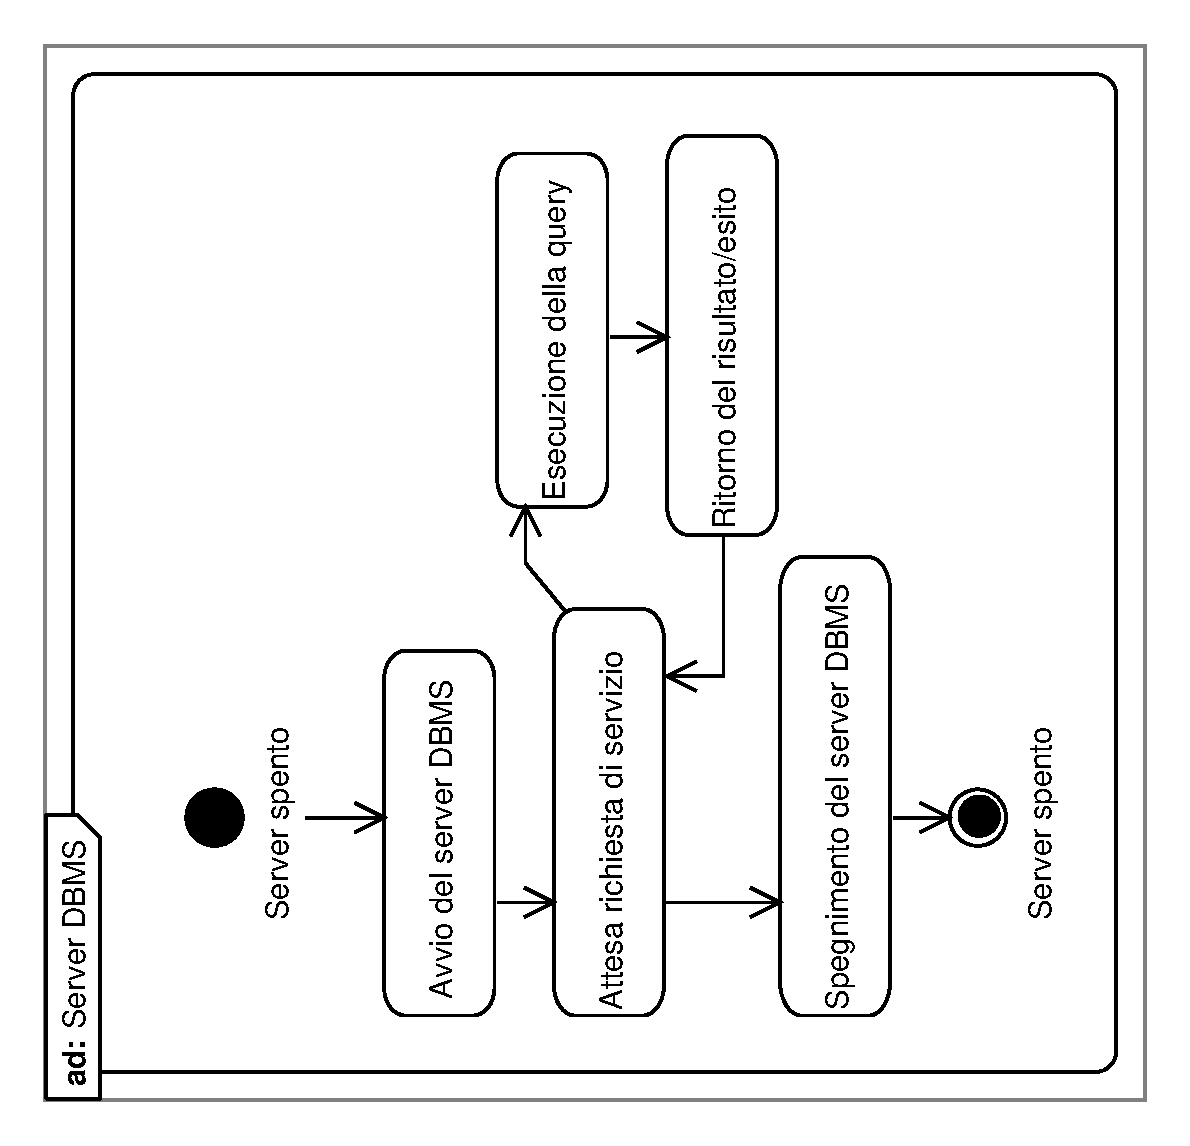
\includegraphics[width=1\textwidth, angle=-90]{Server.eps}
\end{center}

\chapter{Descrizione dei diagrammi di sequenza}
\chapter{Descrizione dei diagrammi di collaborazione}

\chapter{Stime di fattibilit\`a e di bisogno di risorse}
Dopo aver analizzato il problema attraverso schemi progetturali sono state individuate le risorse necessarie  per la realizzazione del prodotto. Attraverso l'utilizzo di software open source siamo riusciti a contenere i costi e contemporaneamente a rendere disponibili tutte le risorse necessarie.
Le risorse necessarie ai nostri componenti per affrontare le varie problematiche di comunicazione, sviluppo del codice, gestione degli archivi, verifica dei documenti e del sistema sono state descritte nel documento Piano di Qualifica. Nella fase di specifica tecnica e successivamente di progettazione verrano utilizzati diagrammi UML delle classi e degli oggetti realizzati con Dia. Lo sviluppo avr\`a luogo singolarmente o in piccoli gruppi a seconda della natura della problematica da affrontare. Il documento/codice avr\`a in ogni modo un unico proprietario incaricato di renderlo pubblico tramite server SVN.
%Parlare ASSOLUTAMENTE di ANTLR e di ANTLRWORKS nonchè di poseidon, eclipse e se la elena per fare la gui utilizza roba esterna dichiararlo...ma poseidon non è + open source!!
\chapter{Tracciamento della relazione componenti-requisiti}

\end{document}

    
